\chapter{Defect-Spin Nano-MR and Optical Detection}
\label{chap:nano-mr}

The \code{spin\_dynamics.nano\_mr} namespace models nanoscale magnetic-resonance
spectroscopy with optically addressable point defects. It currently supports
the diamond NV-minus and 4H-SiC PL6 ground-state sensors, microwave
dynamical-decoupling control, effective optical fluorescence readout, and
statistical, resolved, and diffusing nuclear-spin samples. These models
describe the single-defect
regime introduced by the 2013 proton-detection experiments of
\href{https://doi.org/10.1126/science.1231675}{Staudacher et al.} and
\href{https://doi.org/10.1126/science.1231540}{Mamin et al.}: the detected
nuclear signal is ordinarily a fluctuation variance from a nanometre-scale
volume, not the bulk thermal magnetization assumed by an inductive NMR coil.
The coherent high-resolution layer separately represents clock-referenced fields and
thermally polarized ensemble-NV spectra; it never substitutes those signal
statistics for the single-defect fluctuation model.

\chapterpath{Define a higher-spin defect and surface geometry, construct a
Ramsey or dynamical-decoupling sensing window, connect the filter to a
statistical nuclear bath, and convert sensor population into realistic optical
photon counts.}

\scopebox{Accent}{
\textbf{Use this layer for:} diamond NV-minus and 4H-SiC PL6 ground-state ODMR;
arbitrary sensor and surface orientations; point-dipole electron--nuclear
coupling; Ramsey, Hahn, CPMG, XY4/8/16, KDD, and arbitrary phase-cycled sensing;
ideal or rectangular finite-width pulses; effective addressed-qubit
propagation; contrast-limited Poisson fluorescence; statistical, thermal, or
fixed-polarization nuclear populations; uniform layers, half-spaces, and voxel
densities; multi-isotope Lorentzian spectra; and Gaussian filter-overlap
coherence; exact small nuclear clusters and two-block correlation
spectroscopy; and seeded diffusion, drift, confinement, field correlations,
and spectra; plus scanning-sensor and sensor-array nano-MRI forward models,
depth profiles, nonnegative density reconstruction, sparse point
localization, and uncertainty estimates; plus correlated target/sensor field
processes, rate-equation optical cycling, shot-resolved photon emission, SPAD
detector transfer, and covariance-weighted inversion; plus clocked Qdyne,
synchronized quadrature readout, sensor-memory correlation, coherent thermal
chemical-shift/J spectra, and explicit effective DNP preparation.
}

\scopebox{AccentTwo}{
\textbf{Current limits:} optical-cycle and surface-noise rates are
configurable phenomenological calibrations, not universal NV/SiC constants or
a microscopic surface-chemistry model. The statistical-bath model
prescribes exponentially correlated rotating fields, whereas the trajectory model derives
correlation from classical Brownian trajectories with quantum-matched moment
variance. Exact clusters are limited to small dense Hilbert spaces.
The high-resolution coherent-signal and DNP layers are effective protocol
models, not microscopic ancillary-gate or electron-nuclear polarization-
transfer simulations. Experiment-specific spatial calibration and a quantum
optical excited-state model remain outside the present scope.
}

\section{Defect Hamiltonian, Frames, and Surfaces}

A defect is represented by spin \(S\), a local \(g\) tensor, a zero-field
splitting tensor \(\mathbf{D}\), and an explicit local-to-laboratory rotation.
The ground-state angular-frequency Hamiltonian is
\[
  H =
  2\pi\sum_{ij} D_{ij} S_i S_j
  + 2\pi\frac{\mu_B}{h}
    \mathbf{B}_0^{\mathsf T}\mathbf{R}\mathbf{g}\mathbf{S},
\]
up to the trace convention already included in the supplied ZFS tensor.
For axial spin one, \code{zfs\_tensor\_from\_d\_e} reproduces
\[
  \frac{H_\mathrm{ZFS}}{h}
  =D\left[S_z^2-\frac{S(S+1)}{3}\right]
   +E(S_x^2-S_y^2).
\]
The diamond preset uses the NV-minus ground-state splitting; the SiC preset
uses a configurable PL6 model because defect assignment and surface-dependent
calibration continue to evolve.

\begin{lstlisting}[language=Python]
from spin_dynamics.nano_mr import (
    SurfaceGeometry,
    diamond_nv_minus,
    diagonalize_sensor,
    sic_pl6,
)

surface = SurfaceGeometry(
    point_lab_nm=(0.0, 0.0, 0.0),
    normal_lab=(0.0, 0.0, 1.0),
)
nv = diamond_nv_minus(depth_nm=5.0, axis_lab=(0.0, 0.0, 1.0))
pl6 = sic_pl6(depth_nm=2.0)

odmr = diagonalize_sensor(
    nv,
    b0_vector_tesla_lab=(0.0, 0.0, 5e-3),
)
sensor_position_nm = surface.sensor_position_lab_nm(nv)
\end{lstlisting}

The surface normal points from the host into the sample. A positive sensor
depth therefore places the defect on the opposite side of the plane. All
positions carrying an \code{\_nm} suffix are in nanometres; fields are in
tesla; public ZFS and transition frequencies are in hertz; and Hamiltonians are
in radians per second.

For a point nucleus, \code{point\_dipolar\_hyperfine\_tensor\_hz} returns
\[
  \frac{H_\mathrm{dip}}{h}
  =\mathbf{S}_\mathrm{local}^{\mathsf T}\mathbf{A}
   \mathbf{I}_\mathrm{lab},\qquad
  \mathbf{A}\propto
  \frac{\mathbf{1}-3\hat{\mathbf r}\hat{\mathbf r}^{\mathsf T}}{r^3}.
\]
The inverse-cube dependence and the explicit mixed local/laboratory frame
convention are important when comparing sensor orientations.

\section{Sensing Sequences and Filter Functions}

A \code{SensingSequence} describes the coherent interval between effective
optical preparation and readout. Microwave and nuclear-RF events occupy
separate channels, so concurrent events are representable. Same-channel finite
pulses cannot overlap. Zero-duration microwave pulses compile as exact
rotations; finite rectangular pulses compile as piecewise Hamiltonian steps.

\begin{lstlisting}[language=Python]
from spin_dynamics.nano_mr import (
    cpmg_sequence,
    hahn_echo_sequence,
    xy_sequence,
)

hahn = hahn_echo_sequence(tau_seconds=5e-6)
cpmg8 = cpmg_sequence(8, total_duration_seconds=80e-6)
xy8 = xy_sequence(
    8,
    repetitions=1,
    total_duration_seconds=80e-6,
    pulse_duration_seconds=100e-9,
)
\end{lstlisting}

\subsection{KDD and UDD}
\code{udd\_pulse\_times} uses nonuniform Uhrig timing to cancel successive
orders of low-frequency pure dephasing for ideal pulses. It is a timing
prescription. By contrast, \code{kdd\_sequence} uses equally spaced pulse
centers and a 20-pulse Knill phase cycle to suppress systematic flip-angle and
off-resonance errors while preserving arbitrary transverse states. For ideal
instantaneous pulses under longitudinal dephasing, phase does not change the
scalar toggling function, so KDD-20 has the same filter as an equally spaced
20-pulse train. Its advantage appears in phase-aware finite-pulse or
pulse-error propagation, at the cost of a 20-pulse cycle.

For longitudinal dephasing, each ideal \(\pi\) pulse changes the sign of the
toggling coefficient \(y(t)\). Its Fourier integral and the dimensionless
dephasing filter are
\[
  Y(\omega)=\int_0^T y(t)e^{\ii\omega t}\dd t,
  \qquad
  F(\omega)=\omega^2|Y(\omega)|^2.
\]
During a resonant rectangular finite pulse, the scalar longitudinal
coefficient changes continuously as a cosine. This model captures the first
finite-width correction without claiming a full multilevel lab-frame
simulation.

\begin{lstlisting}[language=Python]
import numpy as np

from spin_dynamics.nano_mr import dephasing_filter_function

omega = 2 * np.pi * np.linspace(10e3, 100e3, 500)
ideal = dephasing_filter_function(cpmg8, omega)
finite = dephasing_filter_function(xy8, omega, pulse_model="finite")
\end{lstlisting}

The addressed-qubit propagator uses
\[
  H(t)=\frac{\delta(t)}{2}\sigma_z+H_\mathrm{control}(t)
\]
in the rotating frame. It is the exact time-domain reference for the filter
layer: in the weak longitudinal-field limit, the accumulated phase agrees with
\(\operatorname{Re}[B_\mathrm{ac}e^{\ii\phi}Y(\omega)]\).

\section{Effective Optical Preparation and Detection}

The optical layer intentionally separates non-unitary initialization and
measurement from coherent spin propagation. \code{OpticalReadoutModel}
contains the bright-state preparation fidelity, initialization time, bright
count rate, dark-state contrast, background rate, readout duration, and dead
time. If \(p_b\) is the bright-state probability, the normalized signal rate is
\[
  f(p_b)=1-C(1-p_b),
\]
and the expected counts after \(N\) repetitions are
\[
  \lambda=N\,t_r
  \left[R_b f(p_b)+R_\mathrm{bg}\right].
\]
Preparation fidelity acts before the count map through
\[
  p'_b=\frac12+(2F_\mathrm{init}-1)\left(p_b-\frac12\right),
\]
and the observed count is drawn from
\[
  n\sim\operatorname{Poisson}(\lambda[p'_b]).
\]

\begin{lstlisting}[language=Python]
from spin_dynamics.nano_mr import (
    OpticalReadoutModel,
    sample_optical_readout,
)

readout = OpticalReadoutModel(
    initialization_fidelity=0.95,
    initialization_seconds=2e-6,
    bright_count_rate_hz=250e3,
    readout_contrast=0.25,
    readout_seconds=400e-9,
    background_count_rate_hz=10e3,
    dead_time_seconds=1e-6,
)

photons = sample_optical_readout(
    readout,
    bright_probability=[0.0, 0.5, 1.0],
    repetitions=100_000,
    sensing_seconds=xy8.total_duration_seconds,
    seed=7,
)
\end{lstlisting}

\begin{figure}[t]
\centering
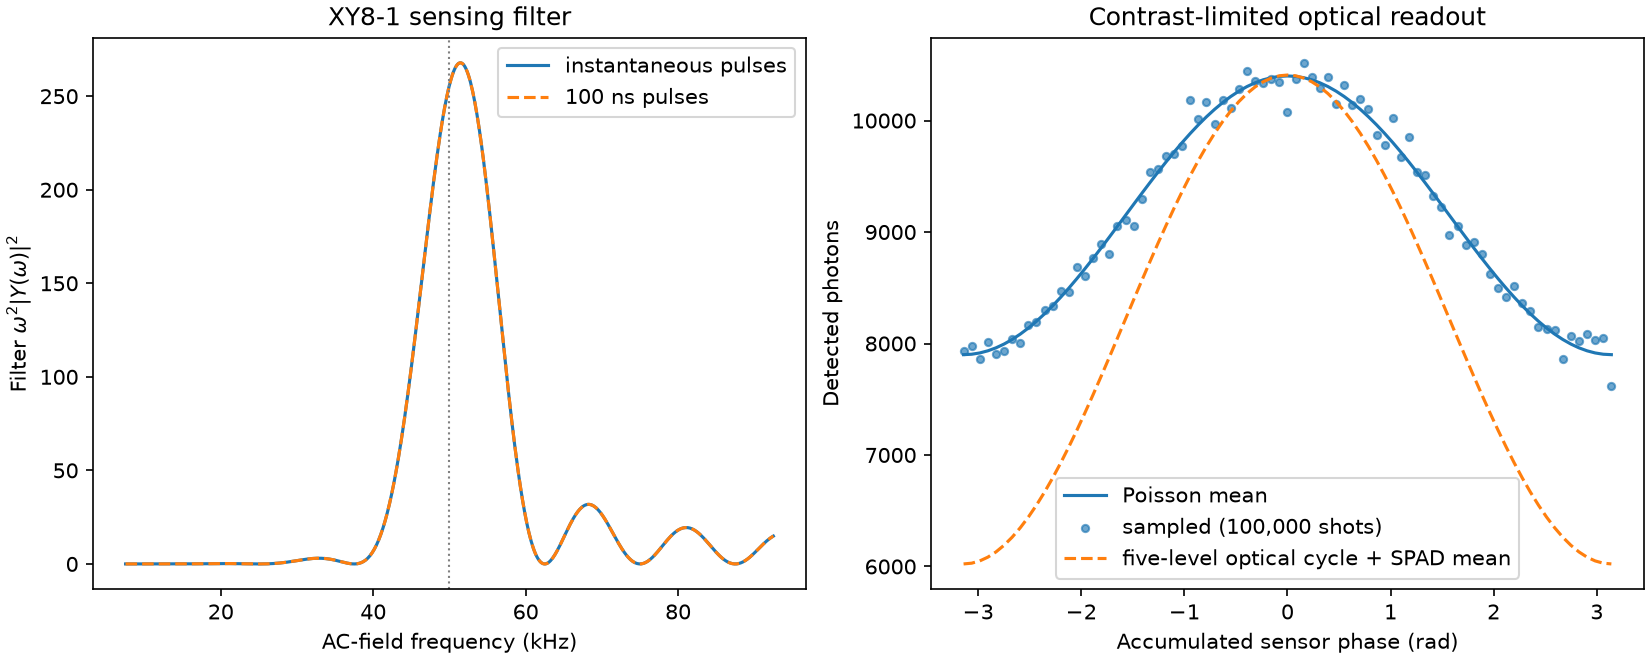
\includegraphics[width=0.98\linewidth]{images/example_nano_mr_xy8_filter_readout.png}
\caption{An XY8 sensing passband with ideal and 100-ns rectangular pulses
(left), and its effective contrast-limited optical photon-count readout
(right). The near-overlap of the filter curves is the expected short-pulse
limit.}
\label{fig:nano-mr-filter-readout}
\end{figure}

This count model is suitable for acquisition-time and shot-noise studies. It
does not model intersystem crossing, metastable shelving, charge conversion,
laser-power saturation, or wavelength-dependent collection. Those require a
separate optical rate-equation layer.

\section{Statistical, Thermal, and Fixed Polarization}

\code{NuclearBathSpecies} records isotope, spin, gyromagnetic ratio,
polarization mode, and field-correlation time. The three population modes are:
\begin{itemize}
  \item \textbf{statistical}: equal Zeeman-level populations;
  \item \textbf{thermal}: Boltzmann weights
    \(p_m\propto\exp[h\gamma_nB_0m/(k_BT)]\);
  \item \textbf{fixed}: the maximum-entropy level distribution whose
    \(\langle I_z\rangle/I\) equals the requested polarization fraction.
\end{itemize}
For any axial population state,
\[
  \langle I_x^2\rangle=\langle I_y^2\rangle
  =\frac{I(I+1)-\langle I_z^2\rangle}{2}.
\]
The statistical-bath model uses this transverse quantum second moment to calculate the rotating
field variance. The mean polarization metadata is retained, but coherent bulk
induction after a tipping pulse is not yet generated.

\begin{lstlisting}[language=Python]
from spin_dynamics.nano_mr import NuclearBathSpecies

proton = NuclearBathSpecies.from_isotope(
    "1H",
    polarization_mode="statistical",
    correlation_time_seconds=150e-6,
)
fluorine = NuclearBathSpecies.from_isotope(
    "19F",
    polarization_mode="thermal",
    temperature_kelvin=300.0,
    correlation_time_seconds=150e-6,
)
\end{lstlisting}

For \(N\) independent nuclei,
\code{species.polarization\_scaling(B0, N)} reports the coherent projection
\(N\langle I_z\rangle\) and the statistical RMS projection
\(\sqrt{N\,\operatorname{Var}(I_z)}\). This keeps the thermal/fixed \(N\)
scaling distinct from statistical \(\sqrt{N}\) scaling without assigning an
artificial lateral volume to an infinite half-space.

\section{Uniform Layers, Half-Spaces, and Voxels}

For a uniform planar sample, the package analytically integrates the dipolar
field over lateral extent. It supports arbitrary relative orientations of
sensor axis, static field, and surface normal. In the collinear limit, a
component of density \(\rho\), thickness \(t\), and closest sensor distance
\(d\) has
\[
  \langle B_\mathrm{ac}^2\rangle
  =\rho\langle I_x^2\rangle
   \left(\frac{\mu_0}{4\pi}h\gamma_n\right)^2
   \frac{\pi}{4}
   \left[d^{-3}-(d+t)^{-3}\right].
\]
For a half-space, the second inverse-cube term vanishes. Field variance
therefore scales as \(d^{-3}\), and RMS field as \(d^{-3/2}\).

\begin{lstlisting}[language=Python]
from spin_dynamics.nano_mr import (
    UniformBathComponent,
    UniformNuclearLayer,
)

sample = UniformNuclearLayer(
    surface,
    (
        UniformBathComponent(proton, number_density_m3=5e28),
        UniformBathComponent(fluorine, number_density_m3=2.5e28),
    ),
    thickness_nm=10.0,  # None selects a half-space
)
\end{lstlisting}

For nonuniform samples, \code{VoxelNuclearSample} accepts \(N\times3\) voxel
centers in nanometres, voxel volumes in \(\mathrm{nm}^3\), and scalar or
per-voxel isotope densities. The calculation is a midpoint dipole sum. Refine
the grid until the result converges, particularly near a shallow sensor where
the \(r^{-6}\) variance kernel changes rapidly.

\section{Multi-Isotope PSD and Filter-Overlap Coherence}

The statistical spectral model assumes the projected nuclear field has correlation
\[
  C_B(t)=\sigma_B^2e^{-|t|/\tau_c}\cos(\omega_Lt).
\]
Its two-sided angular-frequency PSD is
\[
  S_B(\omega)=\sigma_B^2\tau_c
  \left[
    \frac{1}{1+(\omega-\omega_L)^2\tau_c^2}
    +\frac{1}{1+(\omega+\omega_L)^2\tau_c^2}
  \right],
\]
with the explicit normalization
\[
  \sigma_B^2=\int_{-\infty}^{\infty}
  \frac{S_B(\omega)}{2\pi}\dd\omega.
\]
Each isotope contributes peaks at
\(\omega_L=2\pi|\gamma_n|B_0\). Component spectra are retained separately and
summed only for the total sensor field. The result also retains each
component's per-nucleus mean spin projection.

\begin{lstlisting}[language=Python]
from spin_dynamics.nano_mr import simulate_statistical_spectrum

omega = 2 * np.pi * np.linspace(-1.2e6, 1.2e6, 20_001)
spectrum = simulate_statistical_spectrum(
    nv,
    sample,
    b0_vector_tesla_lab=(0.0, 0.0, 20e-3),
    angular_frequencies_rad_s=omega,
)
\end{lstlisting}

For Gaussian noise, the sequence coherence follows directly from the control-sequence
filter:
\[
  \chi=\frac{\gamma_e^2}{2}
  \int\frac{S_B(\omega)|Y(\omega)|^2}{2\pi}\dd\omega,
  \qquad L=e^{-\chi}.
\]
\code{gaussian\_filter\_coherence} evaluates this integral and reports
\(\chi\), \(L\), and the accumulated phase variance. Supply a sorted,
two-sided frequency grid wide and fine enough to resolve both Lorentzian peaks
and filter sidebands.

\begin{figure}[t]
\centering
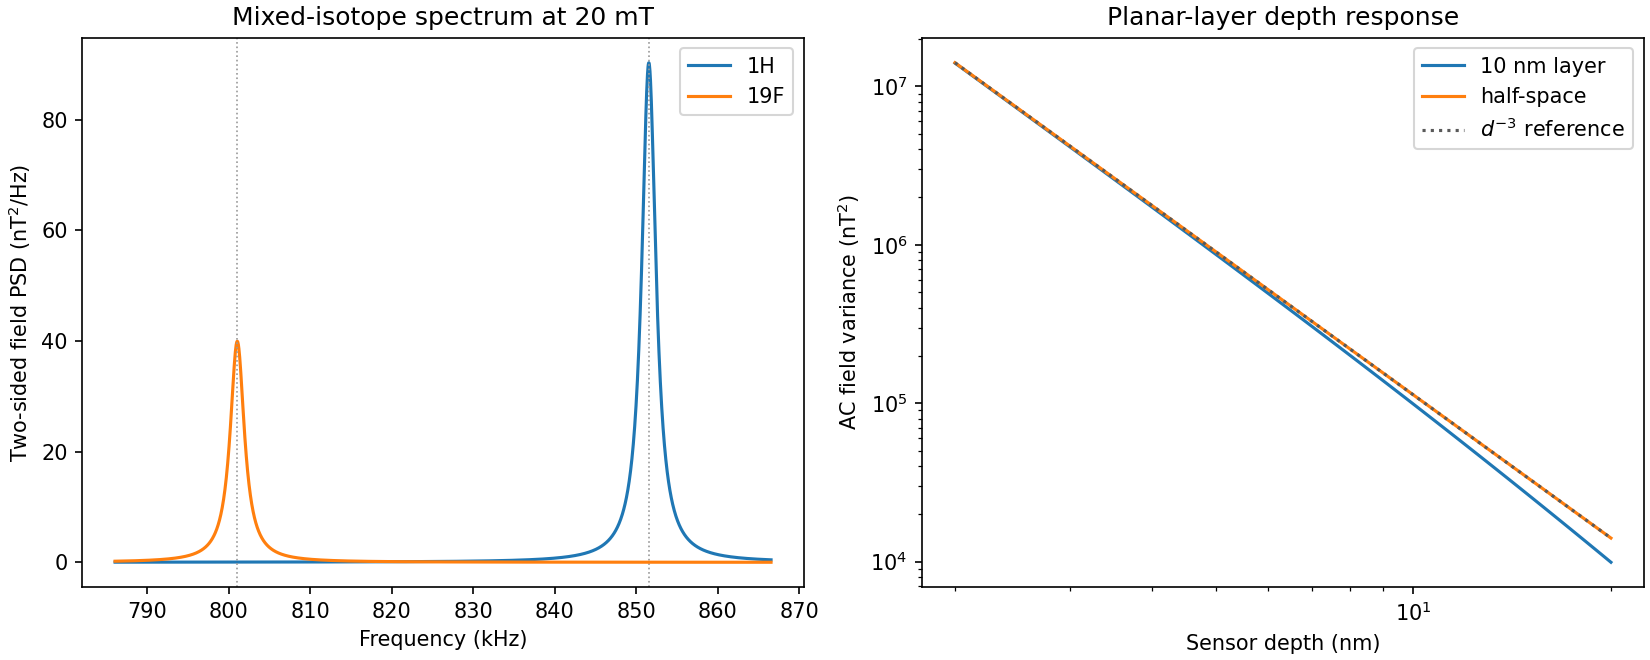
\includegraphics[width=0.98\linewidth]{images/example_nano_mr_statistical_spectra.png}
\caption{Statistical nano-NMR. Left: resolved proton and fluorine
Lorentzians at their isotope-specific Larmor frequencies. Right: finite-layer
and half-space depth response, with the analytic half-space \(d^{-3}\)
variance law.}
\label{fig:nano-mr-statistical}
\end{figure}

Run
\code{python examples/plot\_nano\_mr\_statistical\_spectra.py --output
nano\_mr\_statistical.png} to reproduce
Figure~\ref{fig:nano-mr-statistical}. Run
\code{python examples/plot\_nano\_mr\_xy8\_filter\_readout.py} for
Figure~\ref{fig:nano-mr-filter-readout}.

\section{Exact Resolved-Spin Clusters}

The statistical bath model is appropriate when many weakly coupled nuclei can
be represented by a field correlation function. A few individually resolved
nuclei require a joint density matrix instead. \code{ResolvedSpinCluster}
orders the tensor factors as the defect sensor followed by the nuclei in the
given list. Its angular-frequency Hamiltonian is
\[
\begin{split}
  \mathcal H={}&\mathcal H_\mathrm{defect}
  -2\pi\sum_k\gamma_k
  \left[
    \left(\mathbf 1+10^{-6}\boldsymbol\delta_k\right)^T\mathbf B_0
  \right]\cdot\mathbf I_k \\
  &+2\pi\sum_k\mathbf S^T\mathbf A_k\mathbf I_k
  +2\pi\sum_{j<k}J_{jk}\mathbf I_j\cdot\mathbf I_k
  +\mathcal H_\mathrm{nn}.
\end{split}
\]
Here \(\boldsymbol\delta_k\) is a chemical-shift tensor in ppm,
\(\mathbf A_k\) is the full point-dipole sensor-target tensor, and
\(\mathcal H_\mathrm{nn}\) contains the pairwise nuclear dipolar tensors.
Positive chemical shift increases the bare Larmor frequency in the package
convention. Scalar couplings may be isotropic or field-secular along \(\mathbf B_0\). Nuclear dipolar coupling may retain the full laboratory-frame tensor or use its high-field projection; homonuclear secular pairs retain the energy-conserving transverse flip-flop term. These definitions remain covariant when the complete field and geometry are jointly rotated.

\begin{lstlisting}[language=Python]
from spin_dynamics.nano_mr import (
    NuclearScalarCoupling,
    ResolvedNucleus,
    ResolvedSpinCluster,
    resolved_cluster_hamiltonian,
)

nuclei = (
    ResolvedNucleus.from_isotope(
        "1H", [1.4, 0, 1.4], chemical_shift_ppm=2.1
    ),
    ResolvedNucleus.from_isotope("13C", [2.2, 0, 1.5]),
)
cluster = ResolvedSpinCluster(
    nv,
    nuclei,
    sensor_position_lab_nm=[0, 0, 0],
    scalar_couplings=(NuclearScalarCoupling(0, 1, 140.0),),
)
H = resolved_cluster_hamiltonian(cluster, [0, 0, 20e-3])
\end{lstlisting}

Every public Hamiltonian is in rad/s. Positions remain in nm, fields in T,
couplings and chemical-shift-derived frequency metadata in Hz. The nuclear
gyromagnetic-ratio sign is retained. The resolved cluster is therefore a
coherent quantum model, not a discretized form of the Gaussian statistical-bath model.

\subsection{Dense-System Boundary}

Dense storage and propagation scale exponentially. The default maximum
Hilbert dimension is 64. An NV sensor plus four spin-1/2 nuclei has dimension
\(3(2^4)=48\) and is accepted; five nuclei give dimension 96 and are rejected
before matrix allocation. \code{max\_hilbert\_dimension} can be raised on a
cluster only as an explicit user decision. Raising it does not activate sparse
matrices, a secular cluster expansion, or a cluster-correlation
approximation.

\section{Cross-Listing with Pure ESR}

The ESR and nano-MR modules overlap at one deliberately narrow boundary:
a spin-1/2 center with negligible zero-field splitting. Use the pure ESR
module for conventional radical single-crystal/powder CW spectra, FID and
Hahn response, relaxation, isotropic hyperfine field sweeps, ESEEM, HYSCORE,
and ENDOR. Use nano-MR for higher-spin or finite-ZFS defects, explicit
surfaces, optical initialization/readout, statistical sample layers, and
position-dependent external nuclei.

The two bridge functions have deliberately asymmetric guards:
\begin{itemize}
  \item \code{defect\_sensor\_from\_esr} promotes a compatible pure ESR model
    to a zero-ZFS geometric sensor;
  \item \code{esr\_system\_from\_defect} performs the reverse conversion only
    for spin 1/2 and negligible ZFS.
\end{itemize}
The reverse conversion rejects NV, PL6, and related centers rather than
silently discarding their extra levels or ZFS.

\begin{figure}[t]
\centering
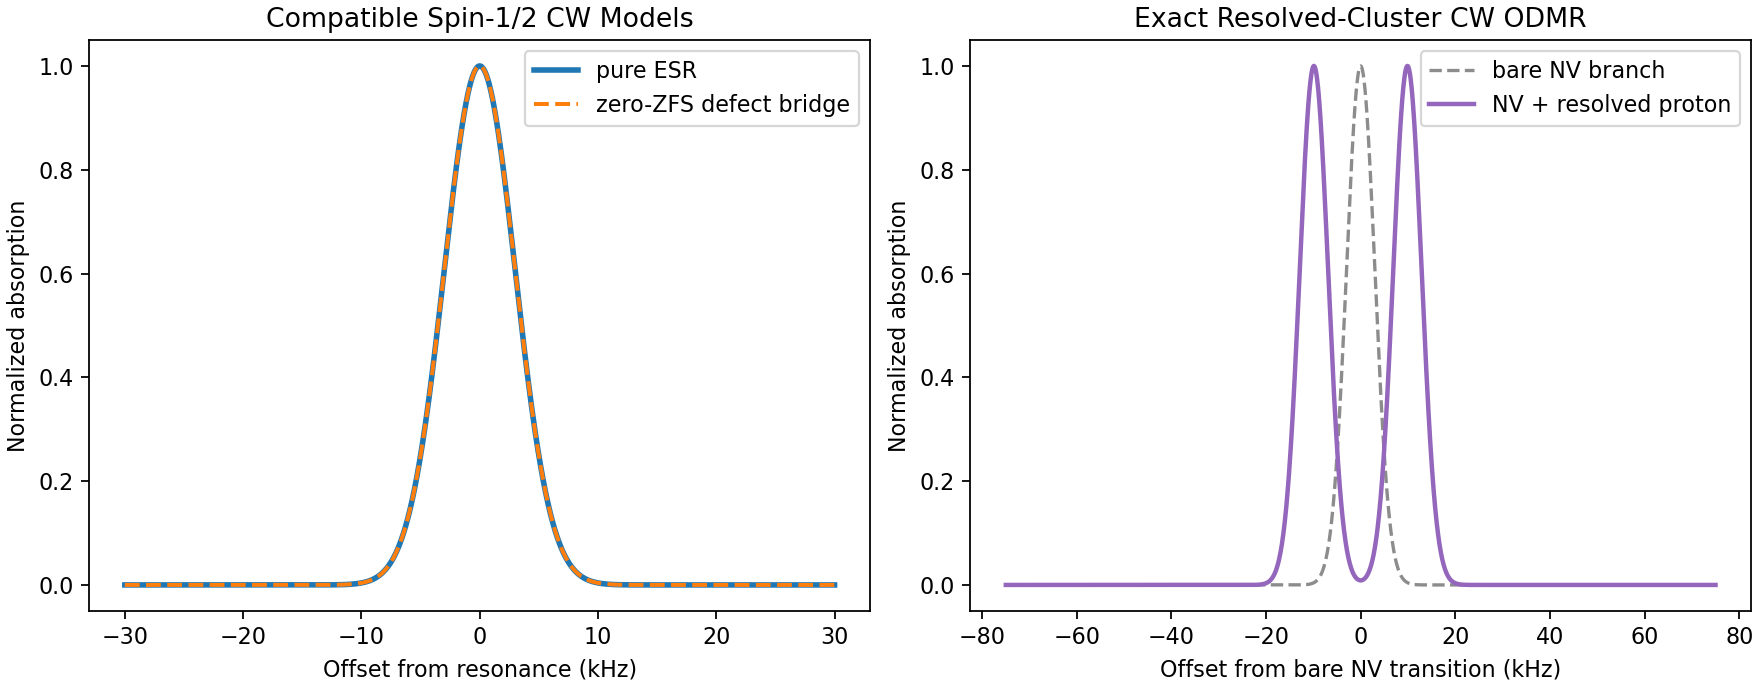
\includegraphics[width=0.98\linewidth]{images/example_esr_nano_mr_cw.png}
\caption{Cross-listed CW models. Left: the pure spin-1/2 ESR spectrum and its
zero-ZFS defect-sensor conversion coincide. Right: the exact cluster backend
resolves the proton-conditioned pair of an NV transition, while the dashed
line is the uncoupled NV branch.}
\label{fig:esr-nano-mr-cw}
\end{figure}

\code{simulate\_resolved\_cw\_spectrum} diagonalizes the complete cluster,
evaluates the embedded electron microwave-drive matrix elements, and broadens
the allowed transitions with the shared ESR line-shape implementation. It is
a frequency-swept transition-strength model: thermal state-population
differences are not included. Optical contrast and photon counting can be
applied afterward with the effective photon-count readout model.

\section{Nuclear RF and Two-Block Correlation}

\code{nuclear\_rf\_hamiltonian} supplies resonant rotating-frame control of
selected nuclei. Its \code{nutation\_hz} convention gives a pi-pulse duration
\(1/(2\nu_1)\). \code{ideal\_nuclear\_rotation} is the corresponding
instantaneous operation for protocol assembly.

The resolved-cluster correlation workflow applies two ideal selective Hahn blocks,
\[
  R_y(\pi/2)\;U(t/2)\;R_x(\pi)\;U(t/2)\;R_y(-\pi/2),
\]
to one bare sensor transition. The complete coupled density matrix is
preserved during a mixing interval. An optional ideal nuclear-RF rotation is
inserted at the mixing midpoint, and the final observable is the lower
sensor-state probability.

\clearpage
\begin{lstlisting}[language=Python]
from spin_dynamics.nano_mr import (
    correlation_spectrum_2d,
    simulate_two_block_correlation,
)

times = np.linspace(0.2e-6, 8e-6, 25)
correlation = simulate_two_block_correlation(
    cluster,
    [0, 0, 20e-3],
    times,
    times,
    mixing_seconds=1e-6,
    nuclear_rf_flip_angle_rad=np.pi,
)
spectrum = correlation_spectrum_2d(correlation)
\end{lstlisting}

\begin{figure}[h]
\centering
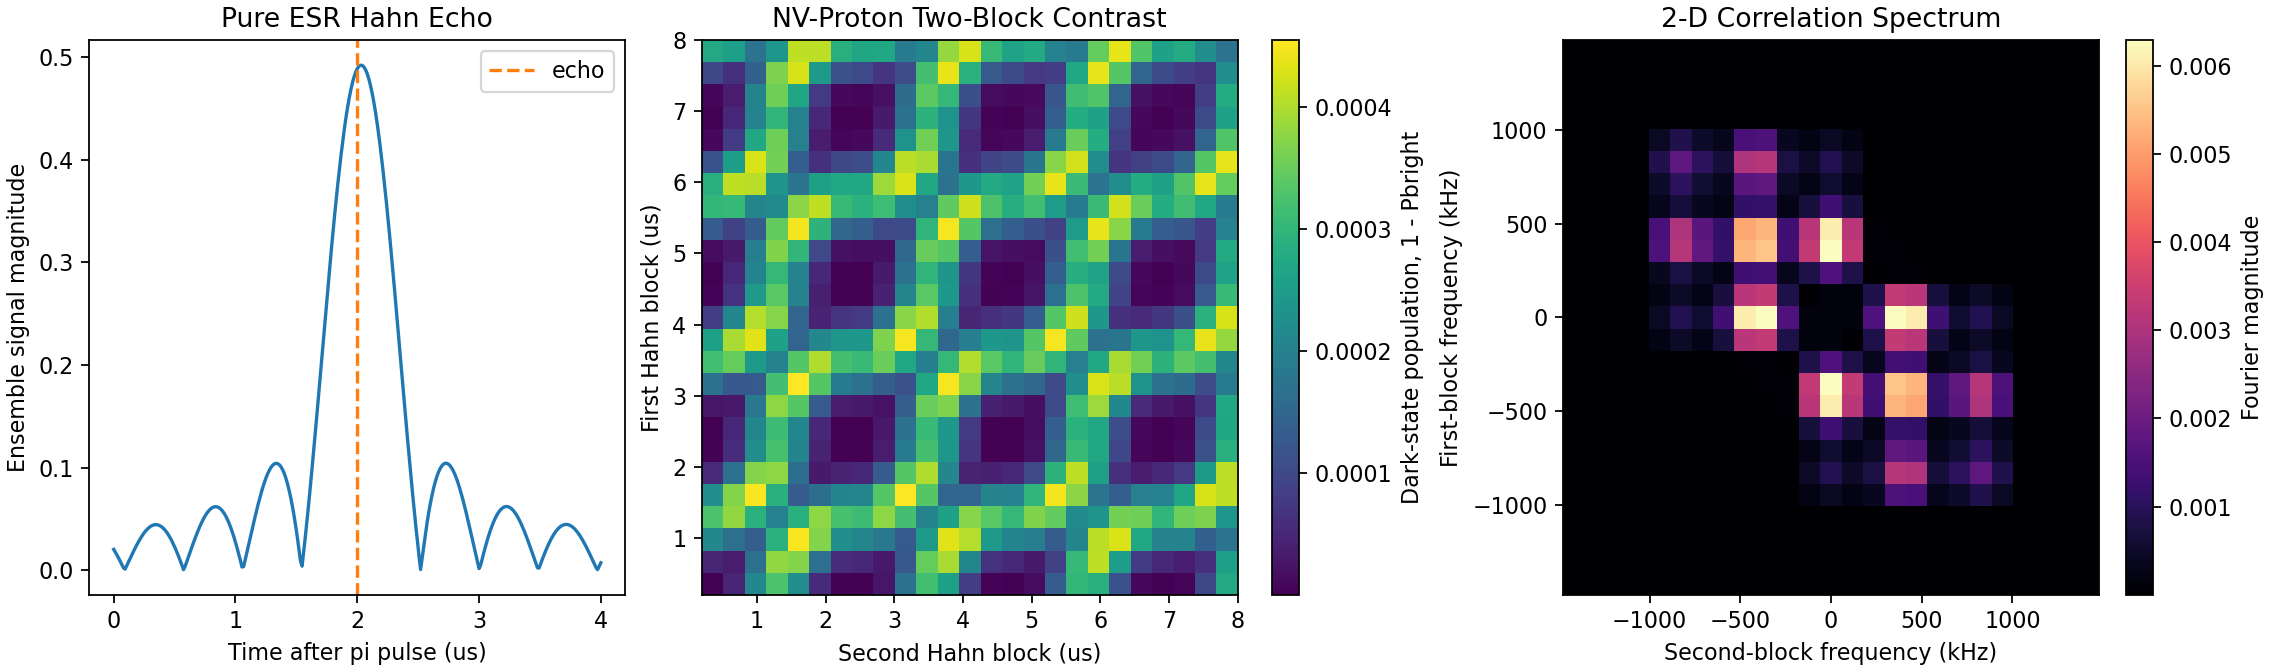
\includegraphics[width=0.98\linewidth]{images/example_esr_nano_mr_pulsed.png}
\caption{Pulsed model cross-listing. A conventional spin-1/2 ESR isochromat
ensemble refocuses at the Hahn echo (left). Exact NV-proton propagation gives
the small residual dark-state population \(1-P_\mathrm{bright}\) (center) and
its windowed 2-D Fourier magnitude (right). The center color scale deliberately
magnifies the approximately \(4.6\times10^{-4}\) modulation.}
\label{fig:esr-nano-mr-pulsed}
\end{figure}

The time axes must be strictly increasing. The 2-D Fourier helper additionally
requires uniform spacing and offers mean removal and a separable Hann window.
These are ideal-pulse results. Shaped-pulse bandwidth, off-resonance pulse
errors, relaxation, sensor reset between blocks, and photon shot noise are not
inserted implicitly; compose those effects explicitly when the experiment
requires them.

The small default modulation is expected rather than a normalization error.
For the 2-nm proton and 20-mT field in
Figure~\ref{fig:esr-nano-mr-pulsed}, the point-dipole tensor norm is
24.2~kHz, its relevant transverse conditional component is 14.8~kHz, and the
proton Larmor frequency is 851.5~kHz. The Hahn blocks refocus the first-order
static longitudinal phase. The remaining noncommuting transverse evolution is
therefore perturbative, with characteristic depth
\[
  \left(\frac{A_\perp}{\nu_L}\right)^2
  =\left(\frac{14.8}{851.5}\right)^2
  \simeq 3.0\times10^{-4}.
\]
The exact two-block calculation spans
\(P_\mathrm{bright}=0.999545\) to nearly 1, or a maximum dark-state
population of \(4.55\times10^{-4}\). Optical readout reduces the fractional
fluorescence modulation further: a readout contrast of 0.25 gives
\(0.25(4.55\times10^{-4})=1.14\times10^{-4}\) relative to the fully bright
signal rate, before background. Resolving it therefore normally requires many
repetitions, phase cycling or differential normalization, and suitable sensor
coherence. Closer nuclei, lower field, or protocols designed to accumulate
the conditional nuclear evolution can produce larger contrast, but may also
invalidate the weak-coupling interpretation.

\section{Diffusing and Confined Liquids}

The diffusion workflow connects the package-wide seeded particle-motion engine to the
nano-MR point-dipole kernel. Each walker represents one nucleus with a random
transverse phase. Its classical moment amplitude is selected so that the phase
ensemble reproduces the quantum transverse second moment of its
\code{NuclearBathSpecies}. The position update is
\[
  \Delta\mathbf r
  =\mathbf v\,\Delta t
  +\sqrt{2D\Delta t}\,\boldsymbol{\xi},
\]
where each component of \(\boldsymbol{\xi}\) is a unit normal variate. The
resulting field at the defect is
\[
  \mathbf B(\mathbf r)
  =\frac{\mu_0}{4\pi r^3}
   \left[
     3\hat{\mathbf r}
       (\boldsymbol{\mu}\mathbin{\cdot}\hat{\mathbf r})
     -\boldsymbol{\mu}
   \right].
\]
This explicit trajectory model complements, rather than replaces, the
prescribed exponential correlation used by the faster analytic statistical-bath
spectrum.

\begin{lstlisting}[language=Python]
from spin_dynamics.nano_mr import (
    NuclearBathSpecies,
    field_autocorrelation,
    field_power_spectral_density,
    simulate_diffusing_dipolar_field,
)

proton = NuclearBathSpecies.from_isotope("1H")
trajectory = simulate_diffusing_dipolar_field(
    initial_positions_nm,
    proton,
    sensor_position_lab_nm=[0, 0, -8],
    static_field_lab_tesla=[0, 0, 20e-3],
    sample_interval_seconds=20e-9,
    sample_count=4096,
    motion_substeps_per_sample=10,
    diffusion_coefficient_m2_s=2e-10,
    bounds_lab_nm=((-20, 20), (-20, 20), (0, 40)),
    boundary="reflect",
    seed=2027,
)
correlation = field_autocorrelation(
    trajectory, normalize=True
)
spectrum = field_power_spectral_density(
    trajectory, segment_length=1024
)
\end{lstlisting}

\begin{figure}[htbp]
\centering
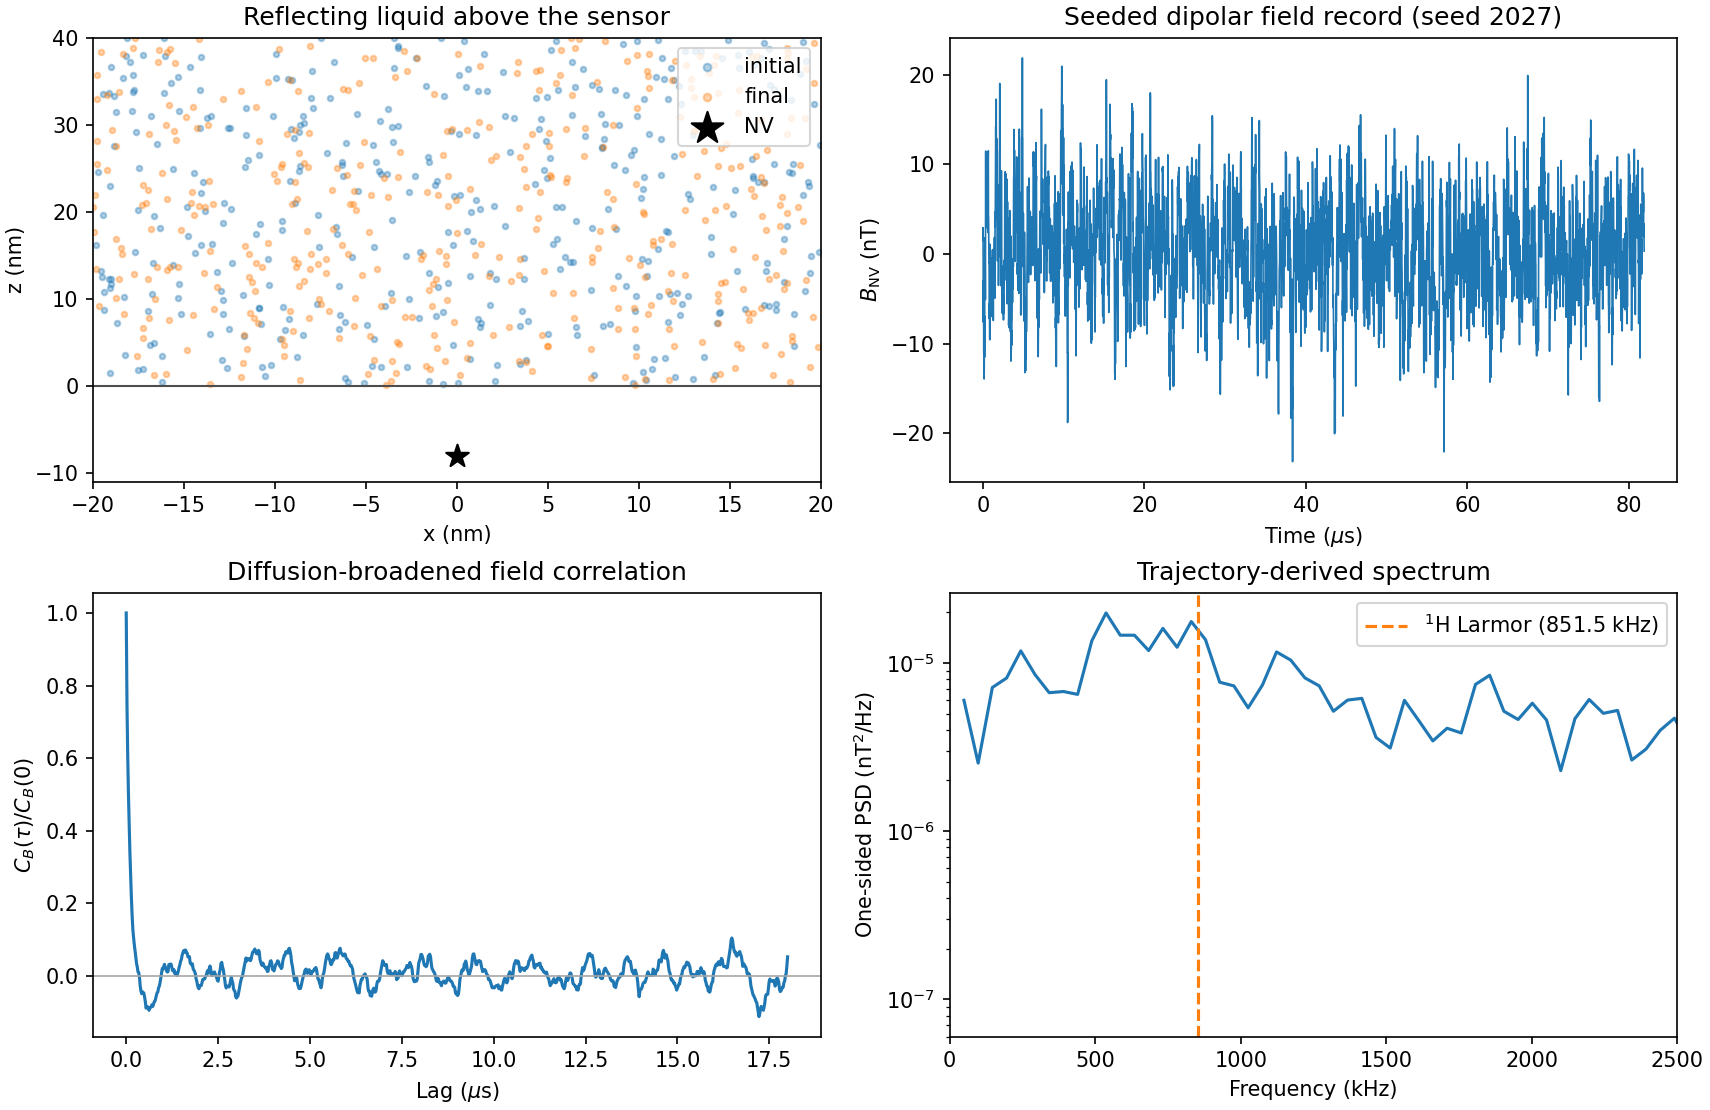
\includegraphics[width=0.98\linewidth]{images/example_nano_mr_diffusing_liquid.png}
\caption{Diffusing-liquid workflow. Seeded protons diffuse inside a
reflecting nanovolume above an 8-nm-deep NV center (upper left), producing a
reproducible sensor-axis dipolar field record (upper right), its normalized
autocorrelation (lower left), and a Welch-averaged one-sided spectrum (lower
right). The deliberately slow confined-liquid diffusivity keeps a broad
proton Larmor feature visible near 851.5~kHz.}
\label{fig:nano-mr-diffusing-liquid}
\end{figure}

Motion integration and field recording have separate time scales.
\code{motion\_substeps\_per\_sample} should make the typical Brownian step
\(\sqrt{2D\Delta t_\mathrm{motion}}\) small compared with the sensor depth and
the narrowest confinement dimension. The field interval can remain longer to
provide a useful spectral span and total record length. The PSD helper uses a
full-record periodogram by default or overlapping Welch averaging when a
segment length is supplied.

Figure~\ref{fig:nano-mr-diffusing-liquid} uses
\(D=2\times10^{-10}\,\mathrm{m^2\,s^{-1}}\). A water-like
\(D\sim2\times10^{-9}\,\mathrm{m^2\,s^{-1}}\) near an 8-nm sensor has a
dimensional decorrelation time \(d^2/D\) of only about 32~ns. Its Larmor
feature can consequently broaden over several megahertz. This loss of
resolution is physical and is one reason diffusion-aware spectral models are
important; see, for example,
\href{https://doi.org/10.1038/s41598-020-76745-4}{Oviedo-Casado et al.}

The validation suite covers four limiting behaviors. A stationary record
retains a constant raw autocorrelation. Unbounded three-dimensional Brownian
motion approaches
\(\langle|\Delta\mathbf r|^2\rangle=6Dt\), imposed flow approaches
\(\langle\Delta\mathbf r\rangle=\mathbf vt\), and reflecting boxes retain
every walker. The Gaussian return propagator
\[
  G(\mathbf 0,t)=(4\pi Dt)^{-3/2}
\]
supplies the expected three-dimensional long-time reference. This algebraic identity is not by itself an end-to-end demonstration that a finite sampled dipolar-field trajectory has reached the asymptotic regime; that requires walker, duration, cutoff, and timestep convergence.

The point-dipole singularity is controlled by an explicit
\code{minimum\_distance\_nm}; choose a physical closest approach such as the
sensor depth plus a surface gap. Displacements computed from wrapped periodic
coordinates contain artificial jumps at the seam, so unwrap those paths
before interpreting their mean-squared displacement.

\section{Scanning Nano-MRI and Reconstruction}

The imaging model treats a scanning sensor and a simultaneous sensor array as the same
linear measurement geometry. A \code{NanoMRScan} stores sensor positions and
one normalized axis per position. \code{raster\_scan} retains serpentine
acquisition order and the indices needed to recover a \((y,x)\) image;
\code{arbitrary\_scan} accepts any ordered path; and \code{sensor\_array}
allows independently oriented detectors.

The forward model keeps two physical observables separate. In coherent
\code{field} mode, a signed moment amplitude multiplies the projected dipolar
kernel
\[
  K_{ij}^{(B)}
  =\frac{\mu_0}{4\pi r_{ij}^3}
   \mathbf n_i^{\mathsf T}
   (3\hat{\mathbf r}_{ij}\hat{\mathbf r}_{ij}^{\mathsf T}-\mathbf 1)
   \hat{\boldsymbol{\mu}} .
\]
In statistical \code{transverse\_variance} mode, the squared transverse
projection maps nonnegative moment variance to field variance. The convenience
builder \code{build\_voxel\_density\_forward\_operator} additionally inserts
the isotope second moment and voxel volume, so its unknown vector is a
physical number density in \(\mathrm{m^{-3}}\).

\begin{lstlisting}[language=Python]
from spin_dynamics.nano_mr import (
    NuclearBathSpecies,
    build_voxel_density_forward_operator,
    planar_voxel_grid,
    raster_scan,
    reconstruct_nonnegative_density,
)

axis = [np.sqrt(2 / 3), 0, np.sqrt(1 / 3)]
scan = raster_scan(
    np.linspace(-12, 12, 25),
    np.linspace(-12, 12, 25),
    z_nm=-8,
    sensor_axis_lab=axis,
)
grid = planar_voxel_grid(
    np.linspace(-10, 10, 17),
    np.linspace(-10, 10, 17),
    z_nm=0,
    thickness_nm=2,
)
operator = build_voxel_density_forward_operator(
    scan,
    grid,
    NuclearBathSpecies.from_isotope("1H"),
    field_tesla=20e-3,
    field_axis_lab=axis,
    minimum_distance_nm=8,
)
result = reconstruct_nonnegative_density(
    operator,
    measured_field_variance_t2,
    regularization=1e-6,
    regularization_order=1,
    noise_std=noise_std_t2,
)
\end{lstlisting}

\begin{figure}[htbp]
\centering
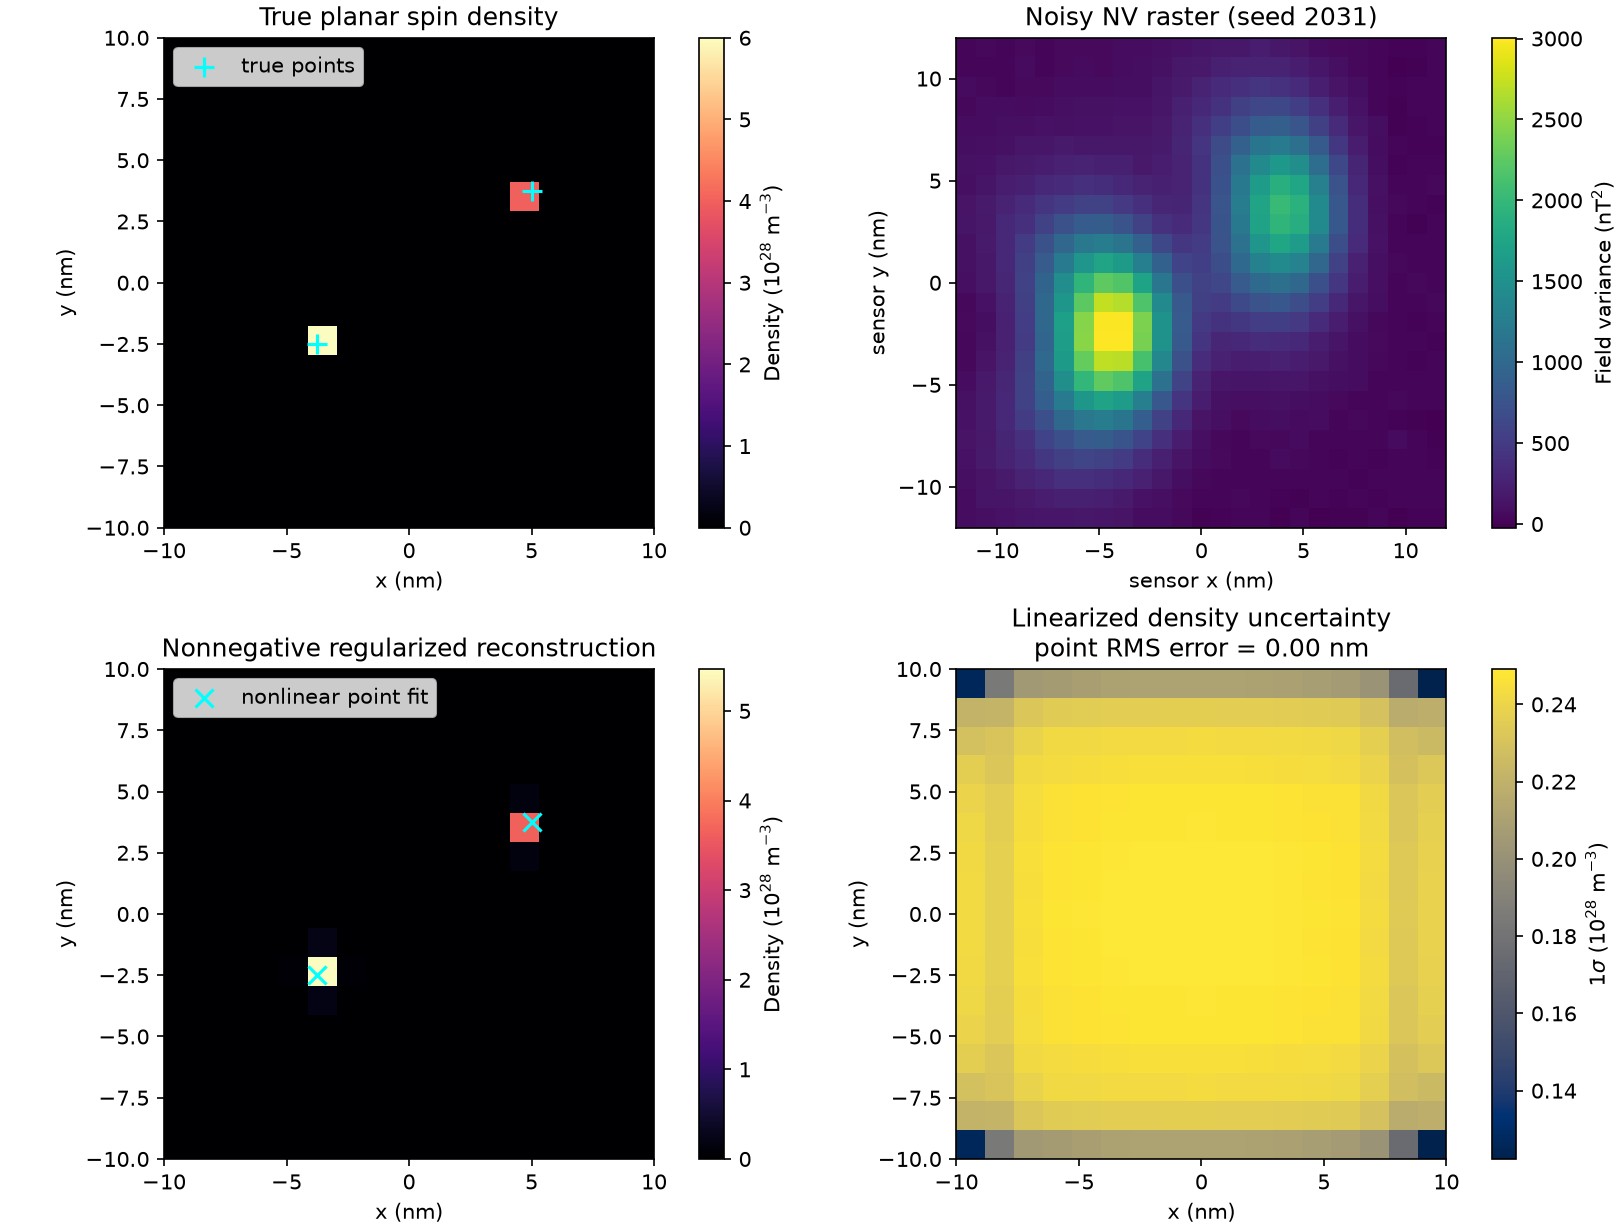
\includegraphics[width=0.98\linewidth]{images/example_nano_mr_scan_reconstruction.png}
\caption{Scanning nano-MRI. Two sparse proton-density voxels (upper
left) produce a seeded noisy statistical-field-variance raster (upper right).
Nonnegative first-difference-regularized inversion recovers the density image
and bounded nonlinear point fitting refines the source positions (lower
left). The local linearized one-standard-deviation density map is shown at
lower right.}
\label{fig:nano-mr-scan-reconstruction}
\end{figure}

The inversion solves
\[
  \underset{\boldsymbol{\rho}\ge0}{\operatorname{argmin}}\;
  \lVert\mathbf K\boldsymbol{\rho}-\mathbf y\rVert_2^2
  +\lambda\lVert\mathbf L\boldsymbol{\rho}\rVert_2^2 .
\]
Projected accelerated gradients enforce nonnegativity. The dimensionless
\code{regularization} value is referenced to the squared spectral norm of the
scaled forward matrix. Penalty order zero shrinks amplitudes, order one favors
piecewise-constant density, and order two favors piecewise-linear density.
For multidimensional source grids, differences are applied along every axis.

The returned covariance is the local Gaussian approximation to the
regularized linear model,
\[
  \operatorname{Cov}(\hat{\boldsymbol{\rho}})
  \simeq
  \sigma^2
  (\mathbf K^{\mathsf T}\mathbf K
   +\lambda\mathbf L^{\mathsf T}\mathbf L)^{+},
\]
with the same internal scaling as the solve. It reports sensitivity and
regularization uncertainty, but not positivity-boundary bias, calibration
error, incorrect sample geometry, or model discrepancy.

\code{build\_depth\_profile\_operator} uses the analytic planar integral from
the analytic statistical-bath model. It maps piecewise-constant density bins above a
surface to field variance for one or more sensor depths. Its one-bin finite
layer agrees exactly with \code{UniformNuclearLayer}; this is preferable to
assuming that a center-point voxel represents an infinite lateral sheet.

For sparse samples, \code{localize\_point\_sources} optionally uses SciPy
bounded least squares to refine point positions and amplitudes. Position and
amplitude standard deviations follow from the local fit Jacobian. They
describe one basin only: source permutations, symmetry-related dipolar
solutions, an incorrect number of points, and other multimodal alternatives
are not summarized by one covariance matrix. The imaging backend therefore supplies a
transparent forward/inverse baseline, not turnkey molecular structure
determination.

\section{Correlated Spin Noise and Physical Optical Detection}

The shot-resolved acquisition layer retains the effective Poisson readout as a fast,
backward-compatible limit while adding the complete stochastic chain
\[
 \text{spin field}\longrightarrow
 \text{sensor population}\longrightarrow
 \text{optical state path}\longrightarrow
 \text{photon arrivals}\longrightarrow
 \text{detector record}.
\]
This separation matters because statistical nuclear polarization is the
signal-generating process, not an interchangeable detector-noise term.
Intrinsic carbon-13, substitutional-nitrogen, surface-electron, and technical
sensor noise remain separately identifiable nuisance processes.

\code{FieldNoiseComponent} supplies an RMS field, correlation time, optional
Larmor frequency, and either an exponential or a power-law envelope. A finite
spatial correlation length additionally correlates nearby scan positions.
The covariance contribution of one component has the form
\[
 C_{ij}=\sigma^2 f(|t_i-t_j|)
 \exp\left(-\frac{|\mathbf r_i-\mathbf r_j|}{\ell}\right),
\]
with the spatial factor omitted for a field common to one scanning sensor.
The power-law option represents the long diffusion tail demonstrated by
\href{https://doi.org/10.1038/s41534-022-00632-1}
{Staudenmaier et al.}; it does not force a Lorentzian line. Surface-bath
components can instead use finite-correlation exponential terms motivated by
\href{https://doi.org/10.1103/PhysRevLett.113.027602}{Myers et al.} and
\href{https://doi.org/10.1103/PhysRevLett.114.017601}{Romach et al.}

\begin{lstlisting}[language=Python]
from spin_dynamics.nano_mr import (
    CorrelatedFieldNoiseModel,
    FieldNoiseComponent,
    sample_correlated_field_noise,
)

noise = CorrelatedFieldNoiseModel((
    FieldNoiseComponent(
        "surface bath", 35e-9, 5e-6
    ),
    FieldNoiseComponent(
        "diffusing target", 12e-9, 25e-6,
        envelope="power_law",
        power_law_exponent=1.5,
        spatial_correlation_length_nm=5,
    ),
))
record = sample_correlated_field_noise(
    noise, shot_times_seconds,
    positions_lab_nm=scan.positions_lab_nm,
    seed=2041,
)
\end{lstlisting}

\code{effective\_sample\_size} reports
\(\operatorname{tr}(C)^2/\operatorname{tr}(C^2)\); correlated shots therefore
do not masquerade as independent averaging. \code{linear\_field\_covariance}
maps independent source-amplitude variances through a linear field operator.

\code{OpticalCycleModel} is a continuous-time rate model containing bright
and dark ground/excited triplet manifolds, the metastable singlet, and an
optional NV-zero charge state. Its radiative, intersystem-crossing,
ionization, and recombination rates determine transient fluorescence,
initialization, singlet shelving, optical spin pumping, and charge blinking.
The five-level form follows the time-resolved analysis of
\href{https://doi.org/10.1364/JOSAB.33.000B28}{Gupta et al.}; the optional
charge rates represent the observed photoionization dynamics of
\href{https://doi.org/10.1088/1367-2630/15/1/013064}{Aslam et al.}
Literature rates are illustrative presets, not universal defect constants.

\code{SPADDetectorModel} then transfers emitted photons through collection
efficiency, background and dark arrivals, paralyzable or nonparalyzable dead
time, one-generation exponential afterpulsing, and timing jitter.
\code{sample\_time\_resolved\_optical\_readout} returns every shot's emitted
and detected counts plus detected arrival times. Its Fano factor exposes
under- or overdispersion that an aggregated Poisson mean hides.

\begin{figure}[htbp]
\centering
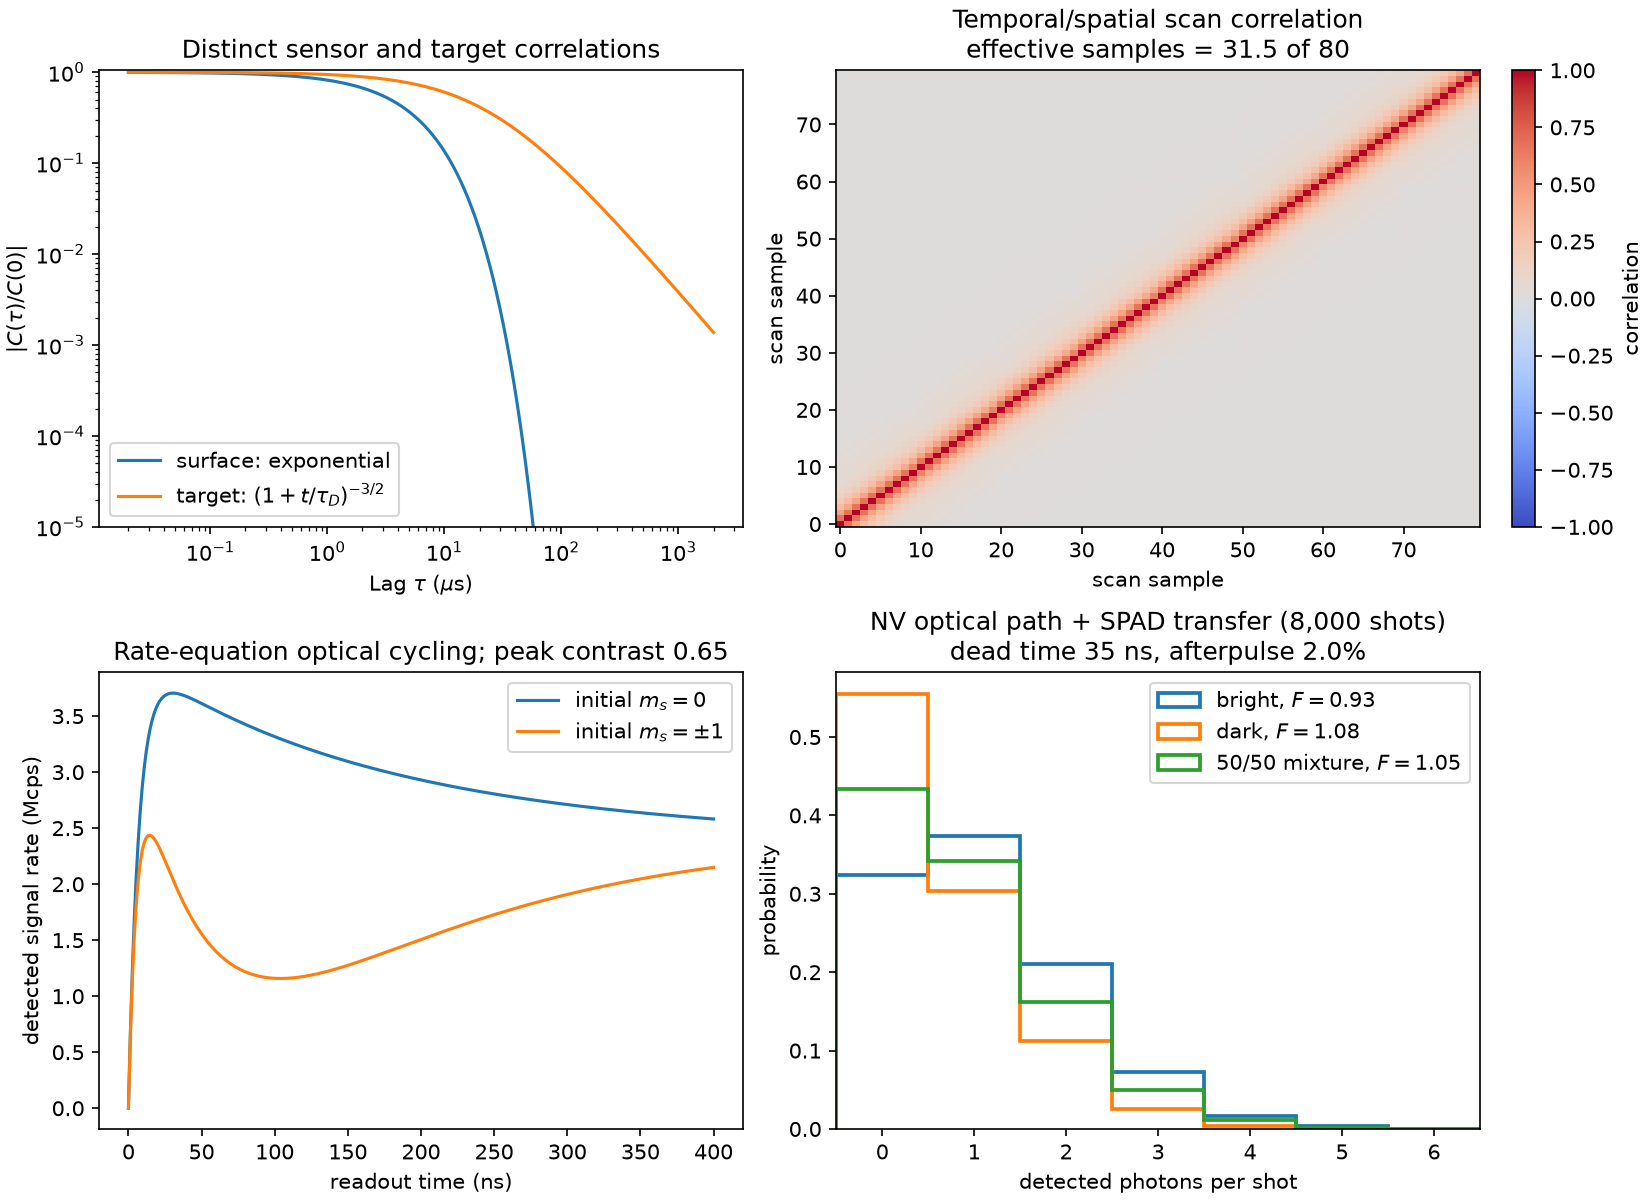
\includegraphics[width=0.98\linewidth]{images/example_nano_mr_realistic_noise.png}
\caption{Stochastic acquisition. Exponential sensor-surface noise
and a long-tailed diffusing target remain distinct (upper left). Their
temporal and spatial correlations reduce 80 scan samples to about 32
effective independent samples (upper right). A configurable optical rate
model gives transient bright/dark fluorescence (lower left), after which an
explicit SPAD produces the conditional and mixed photon-count distributions
(lower right).}
\label{fig:nano-mr-realistic-noise}
\end{figure}

For imaging, \code{reconstruct\_nonnegative\_density} now accepts a positive-
definite \code{noise\_covariance} and solves the generalized least-squares
problem
\[
 \underset{\boldsymbol{\rho}\ge0}{\operatorname{argmin}}\;
 (\mathbf K\boldsymbol{\rho}-\mathbf y)^{\mathsf T}
 \mathbf C^{-1}
 (\mathbf K\boldsymbol{\rho}-\mathbf y)
 +\lambda\lVert\mathbf L\boldsymbol{\rho}\rVert_2^2 .
\]
The original scalar \code{noise\_std} remains available, and the two noise
arguments are mutually exclusive. The returned covariance is conditional on
the supplied calibration and remains a local regularized approximation; it
does not marginalize uncertain optical rates, geometry, or model discrepancy.
The point-source localizer accepts the same covariance for its whitened
nonlinear residual. The scan example enables both paths with
\code{--correlated-noise}. The XY8 example uses \code{--rate-readout} to
overlay the optical-cycle/SPAD mean without removing the original effective
Poisson calculation.

\section{Clocked High-Resolution Protocols}

The high-resolution backend adds coherent, clock-referenced acquisition while preserving the
statistical-bath, exact-cluster, trajectory, and optical APIs. Qdyne and
synchronized readout separate frequency resolution from one sensor
coherence window for a phase-coherent signal, as demonstrated by
\href{https://doi.org/10.1126/science.aam5532}{Schmitt et al.} and
\href{https://doi.org/10.1126/science.aam7009}{Boss et al.}
They do not make an intrinsically statistical nanoscale bath phase coherent.

For a field \(B\cos(\omega t+\phi)\), the control sequence supplies
the complex response
\[
 Y(\omega)=\int_0^{T_s}y(t)e^{i\omega t}\,dt ,
\qquad
 \Phi_n=\gamma_eB\,\operatorname{Re}
 \left[e^{i(\omega t_n+\phi)}Y(\omega)\right].
\]
Sensor coherence enters the measured visibility rather than the accumulated phase, \(s_n=C_s\sin(\Phi_n+\phi_a)\). \code{QdyneProtocol} combines that sensing sequence with a repetition interval, reference frequency, analysis contrast, \code{ClockModel}, and \code{HighResolutionBudget}. \code{simulate\_qdyne} reports nominal and
perturbed timestamps, the complex filter response, expected bright
probabilities, the unsigned real-record baseband spectrum, and an optional
seeded reuse of \code{OpticalReadoutModel}.
\code{simulate\_synchronized\_readout} returns both analysis quadratures, so
the beat-frequency sign is retained.

\begin{lstlisting}[language=Python]
from spin_dynamics.nano_mr import (
    ClockModel, HighResolutionBudget,
    QdyneProtocol, simulate_qdyne,
    xy_sequence,
)

signal_hz = 200e3
sequence = xy_sequence(
    8, 1, 8 / (2 * signal_hz)
)
budget = HighResolutionBudget(
    sensor_coherence_seconds=100e-6,
    sample_coherence_seconds=1.2,
    diffusion_correlation_seconds=2.0,
    memory_coherence_seconds=3.0,
)
protocol = QdyneProtocol(
    sequence,
    repetition_interval_seconds=1e-3,
    reference_frequency_hz=signal_hz - 7,
    budget=budget,
    clock=ClockModel(
        interval_fractional_frequency_instability=1e-9
    ),
)
result = simulate_qdyne(
    protocol,
    signal_frequency_hz=signal_hz,
    field_amplitude_tesla=8e-9,
    sensor_gamma_rad_s_t=2*np.pi*28e9,
    shot_count=4096,
    seed=2042,
)
\end{lstlisting}

The clock model keeps a static fractional frequency offset, independent
interval fractional-frequency instability, and trigger jitter separate.
Likewise the resolution budget does not hide unrelated physics in one
``effective \(T_2\).'' Sensor coherence acts within a sensing block. Sample
transverse coherence and diffusion attenuate correlations across clocked
shots. Ancillary-memory coherence applies only to stored correlations.
The Fourier-bin spacing is \(1/T_{\rm record}\), but sample coherence, diffusion, clock stability, record duration, signal-to-noise, and the Nyquist alias remain physical resolution limits. Results report the raw detuning, Nyquist-folded beat, and alias order separately. Clock-perturbed coherent FIDs use one actual elapsed-time axis for carrier phase, relaxation, diffusion, and scalar-coupling modulation.

\subsection{Relation to ENDOR Qdyne}
The current simulator is a conventional classical-field Qdyne forward model:
it applies a microwave sensing-sequence filter to a coherent field and samples
the response against an external clock.
\href{https://doi.org/10.1038/s42005-023-01419-2}{Meinel et al.}
instead introduce ENDOR Qdyne. Phase-coherent nuclear RF pulses map the target
transverse component to \(I_z\), an electron Ramsey block senses the static
\(A_{zz}S_zI_z\) interaction, and a final RF pulse returns the target to the
transverse plane. This removes the need for microwave refocusing pulses on the
nuclear-Larmor timescale. KDD appears in their conventional DD-Qdyne
comparison; it is not the source of ENDOR Qdyne's high-field reach.

The present model covers clocked down-conversion, sensing filters, visibility,
aliases, and classical coherent envelopes. It does not propagate the paper's
RF basis mapping, target-spin back-action, hyperfine-conditioned phase kicks,
or initialization/charge-error linewidth. Reproducing those results requires
a coupled electron--nuclear cycle map with optical reset and nuclear-state
carryover between shots.

\code{sensor\_memory\_correlation} implements an effective two-block
correlation,
\[
 S(t)=C_0F_{\rm tr}F_{\rm ret}C_s^2
 e^{-t/T_{2,\rm sample}}
 e^{-t/\tau_D}
 e^{-t/T_{2,\rm mem}}
 \cos(2\pi ft+\phi).
\]
It returns the sample, diffusion, and memory envelopes separately, along with
transfer/retrieval fidelity and the two finite-sensor-\(T_2\) block contrast.
This is a transparent protocol-level model, not a microscopic ancillary-gate
error simulation.

\begin{figure}[htbp]
\centering
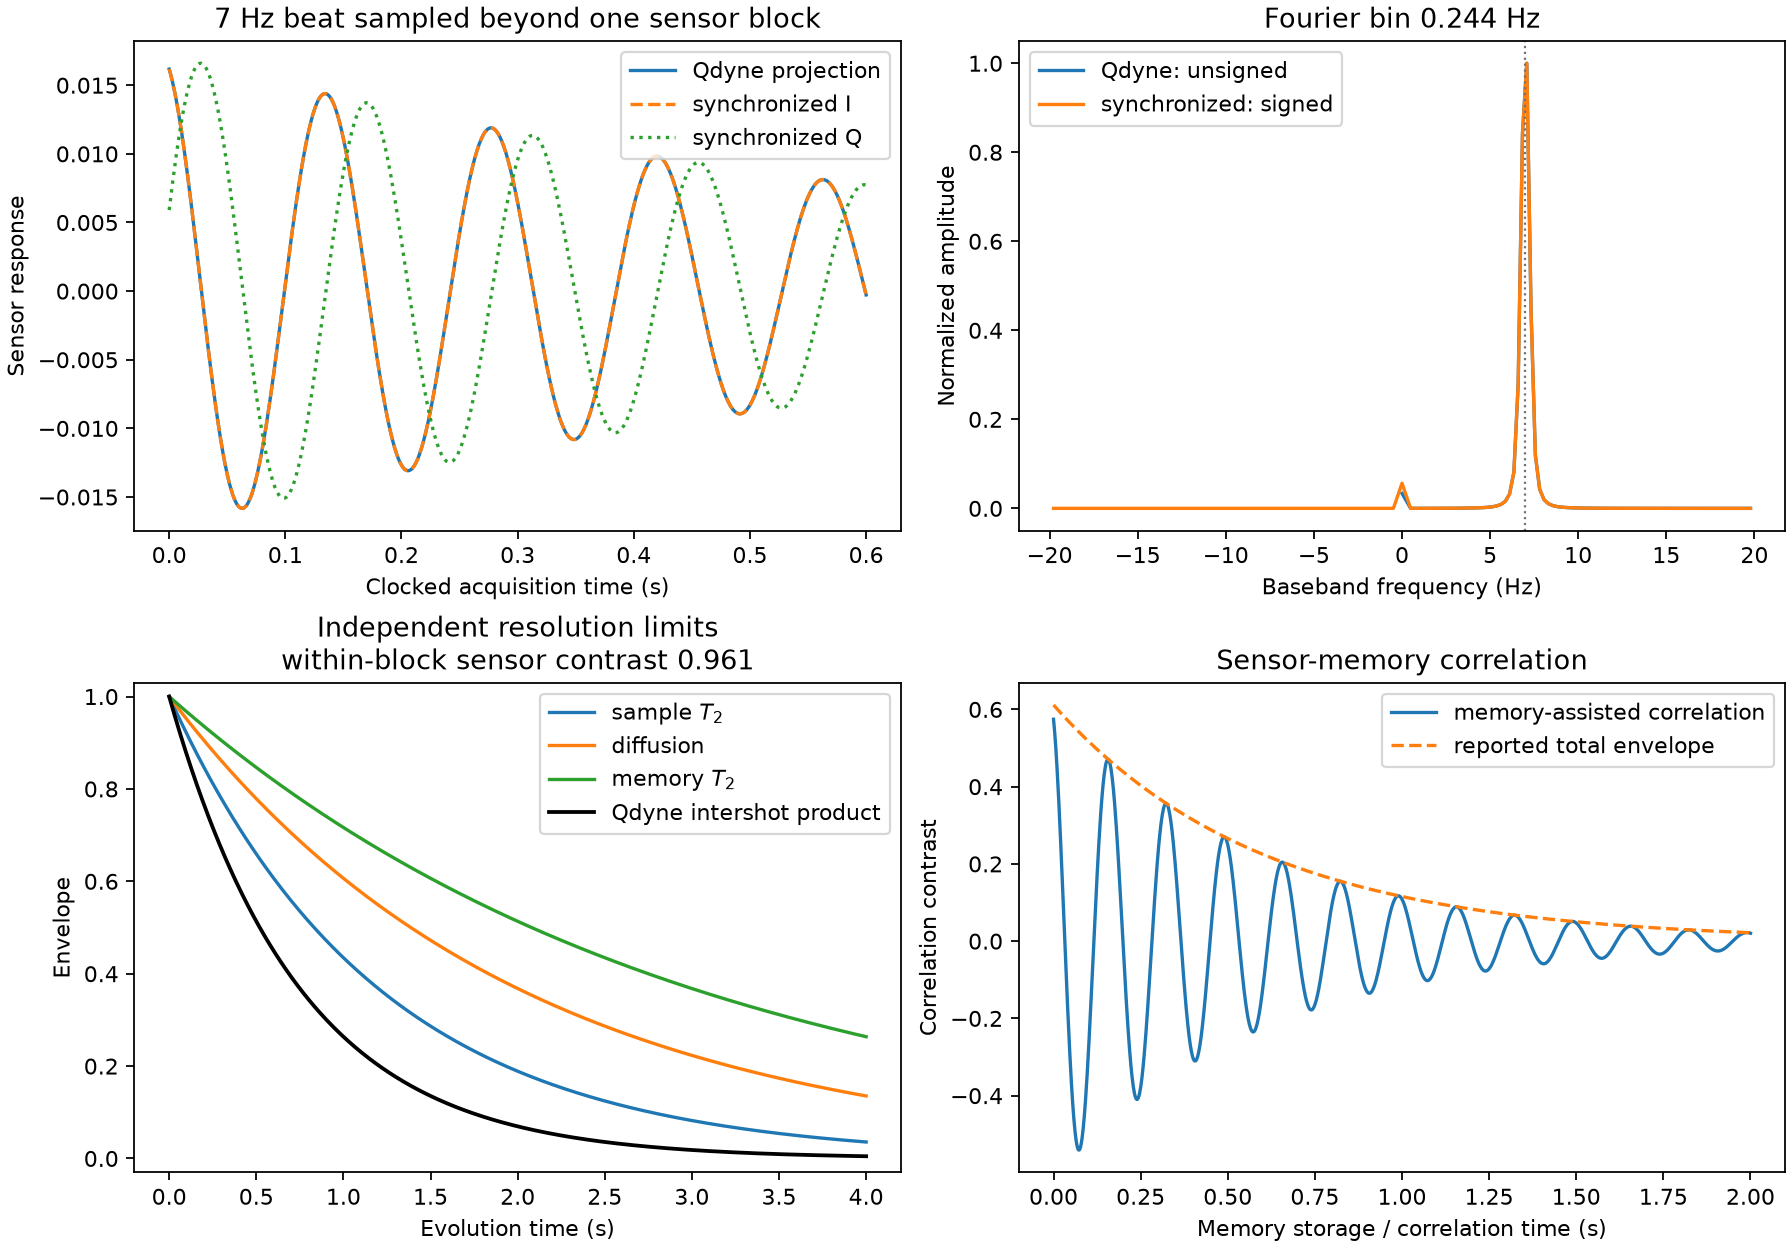
\includegraphics[width=0.98\linewidth]{images/example_nano_mr_qdyne.png}
\caption{Clocked acquisition. Qdyne samples a coherent field beyond
one sensor block, while synchronized I/Q analysis preserves both quadratures
(upper left). Their baseband spectra resolve the clock-referenced beat with
bin spacing set by total record time (upper right). Sensor, sample, diffusion,
and memory envelopes remain independently visible (lower left), and the
sensor-memory protocol reports its oscillatory correlation and total
envelope (lower right).}
\label{fig:nano-mr-qdyne}
\end{figure}

\section{Coherent Thermal, Chemical-Shift/J, and DNP Models}

Thermally polarized ensemble-NV spectroscopy can resolve chemical shifts and
scalar couplings, as demonstrated by
\href{https://doi.org/10.1038/nature25781}{Glenn et al.}; its coherent mean
signal must not be conflated with the statistical variance ordinarily
detected by a single shallow NV. \code{CoherentNMRSite} therefore describes a
first-order coherent site with isotope, chemical shift, complex amplitude,
sample \(T_2\), and weak scalar couplings. A thermally grounded amplitude can
be taken directly from
\code{NuclearBathSpecies.polarization\_scaling}.

For site \(k\), the fast coherent backend evaluates
\[
 s_k(t)=A_k e^{-t/T_{2,k}}e^{-t/\tau_D}
 e^{i2\pi(\nu_k-\nu_{\rm ref})t+i\phi_k}
 \,\prod_j\cos(\pi J_{kj}t),
\qquad
 \nu_k=|\gamma_kB_0|(1+\delta_k10^{-6}).
\]
Repeated equal couplings are combined into their binomial degeneracies:
two equivalent spin-one-half partners give a 1:2:1 triplet and three give a
1:3:3:1 quartet. \code{simulate\_coherent\_nmr\_spectrum} returns the complex
FID, FFT, and explicit component frequencies and weights. Strong coupling,
anisotropic shifts, and exact sensor-target dynamics remain the domain of the
the \code{ResolvedSpinCluster} backend.

\code{DNPModel} is optional and explicit. During pumping,
\[
 P(t)=P_{\rm ss}+(P_0-P_{\rm ss})e^{-t/T_{\rm build}},
\qquad
 P_{\rm ss}=\operatorname{clip}(\epsilon P_{\rm th},-1,1),
\]
whereas after pumping the state relaxes toward \(P_{\rm th}\) with nuclear
\(T_1\). \code{dnp\_polarization} reports thermal, steady-state, and
time-dependent polarization; it does not silently alter optical contrast,
sensor coherence, or detector efficiency. It is an effective preparation
law, not a microscopic electron-nuclear transfer calculation.

\begin{figure}[htbp]
\centering
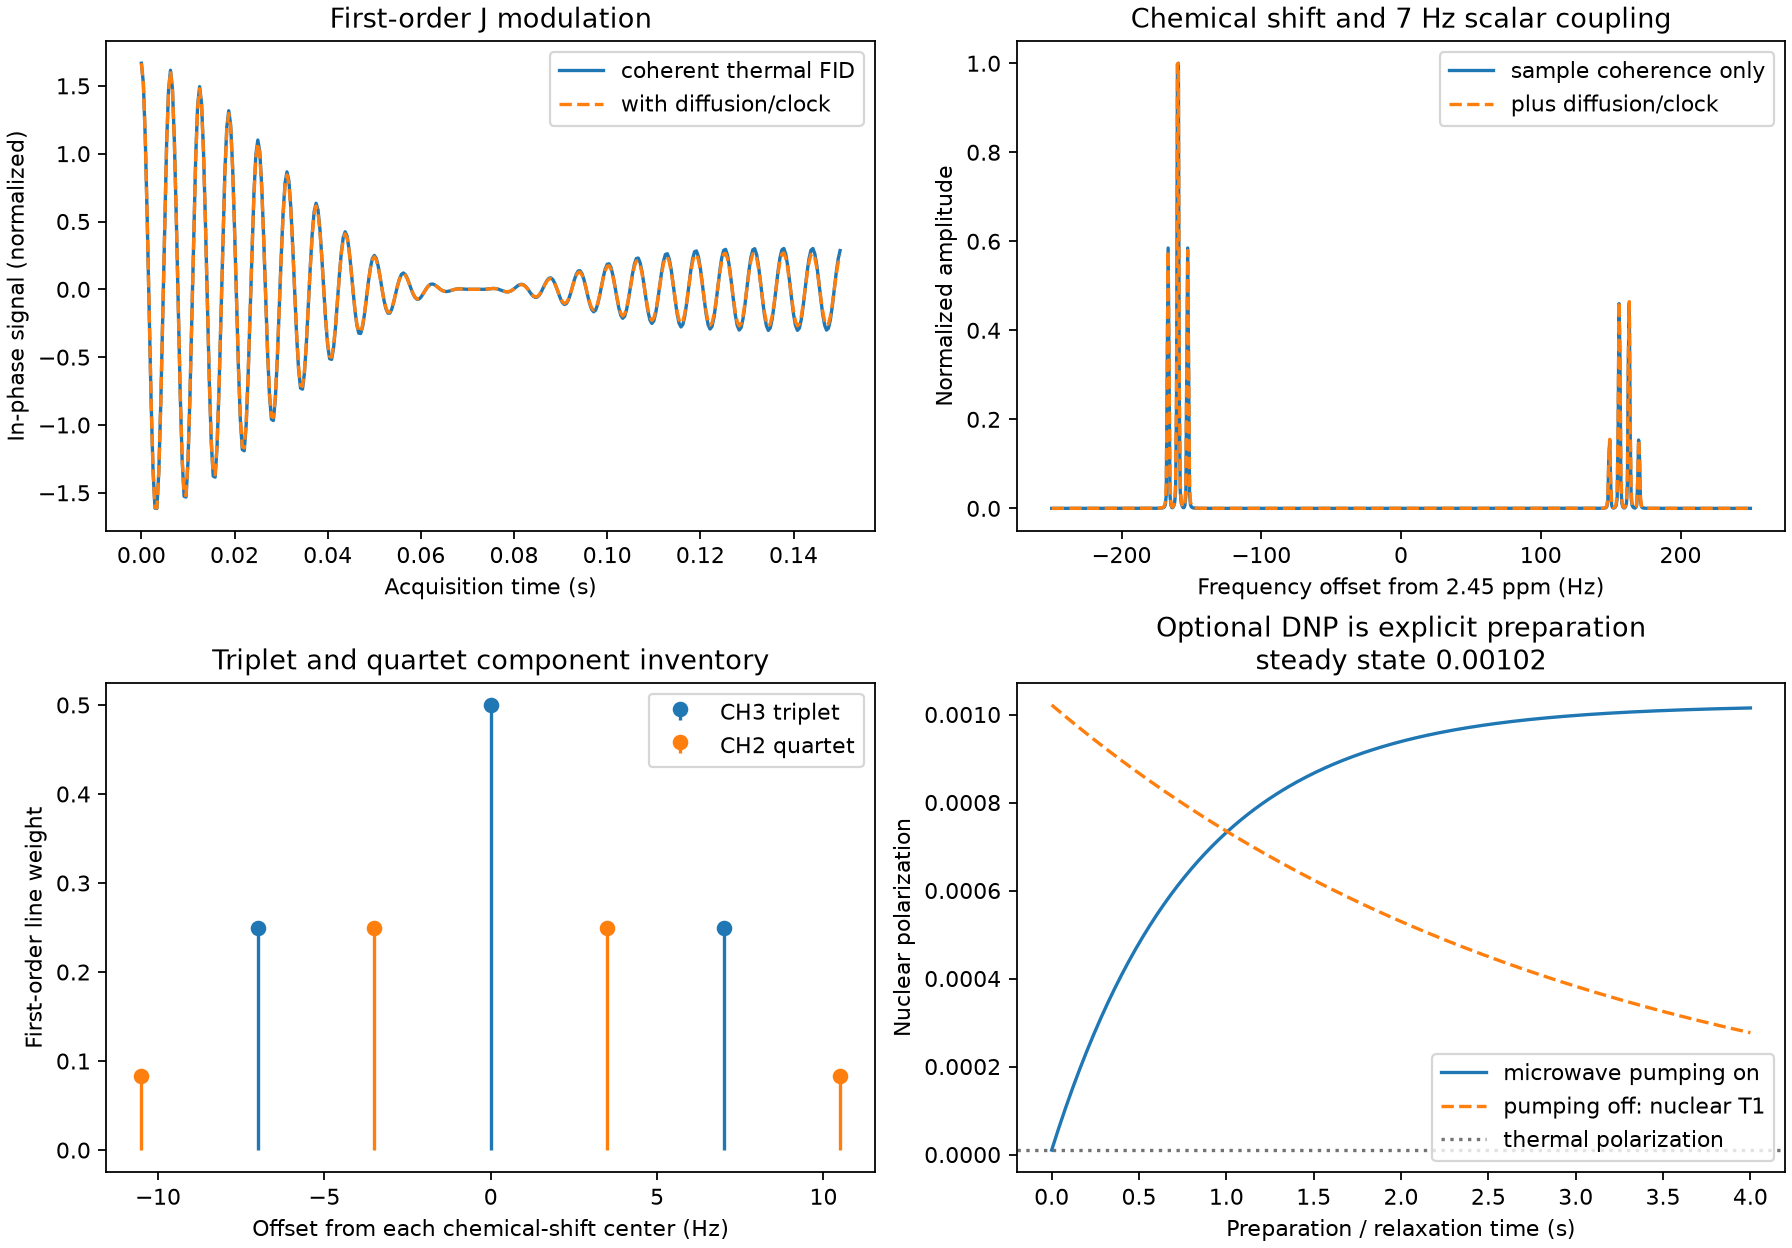
\includegraphics[width=0.98\linewidth]{images/example_nano_mr_chemical_shift_j.png}
\caption{Coherent thermal high-resolution spectroscopy. A thermally grounded
FID displays first-order scalar-coupling modulation (upper left), and its
spectrum resolves two chemical-shift sites and 7-Hz multiplets (upper right).
The explicit component inventory shows a triplet and quartet (lower left).
Optional DNP appears as bounded polarization build-up followed by nuclear-
\(T_1\) decay, not as an unexplained readout gain (lower right).}
\label{fig:nano-mr-chemical-j}
\end{figure}

\section{Unified Experiments, Archives, and Adaptive Qdyne}

Phase~8 connects two common nano-MR calculations to the package-wide
declarative experiment facade. \code{NanoMRStatisticalSpectrum} describes an
analytic planar statistical bath, while \code{NanoMRQdyne} describes a
clocked coherent tone. Their shared physical inputs are compact nested specs:
\code{NanoMRSensor}, \code{NanoMRLayer}, \code{NanoMRBathComponent}, and the
optional effective \code{NanoMROpticalReadout}. The planner requires an
explicit defect sensor and, for a statistical spectrum, an explicit layer.
It rejects overlapping finite XY pulses and reports fields that the selected
workflow would ignore. With optical readout enabled, the repetition interval
must contain initialization, sensing, readout, and detector dead time.

\begin{lstlisting}[language=Python]
from spin_dynamics.experiment import (
    Experiment, Hardware, NanoMROpticalReadout,
    NanoMRQdyne, NanoMRSensor,
)

experiment = Experiment(
    sequence=NanoMRQdyne(
        signal_frequency_hz=2e6,
        field_amplitude_tesla=20e-9,
        shot_count=1024,
        sensing_duration_seconds=2e-6,
        repetition_interval_seconds=20e-6,
        reference_frequency_hz=1.999e6,
        seed=11,
    ),
    hardware=Hardware(
        nano_mr_sensor=NanoMRSensor(depth_nm=5),
        nano_mr_optical_readout=NanoMROpticalReadout(),
    ),
)
print(experiment.plan().report())
record = experiment.run()
record.save("qdyne.npz")
\end{lstlisting}

Friendly JSON and TOML configurations round-trip nested sensors, layers, and
multi-isotope component tables. The saved NPZ archive contains the native
spectrum or clock record, optional photon counts, canonical experiment spec,
randomness status, and implementation/environment provenance. This is useful
for reproducibility, but a matching archive fingerprint is a numerical
identity check rather than validation against a physical instrument.

The planner also supplies deterministic work-unit and memory models. The
statistical path scales with frequency points times isotope components; the
Qdyne path includes the clock record, XY response, and real FFT. A loose
wall-time gate catches accidental algorithmic regressions. Neither the
host-calibrated estimate nor that regression ceiling is a portable performance
claim.

\code{NanoMRQdyneAdapter} adds adaptive design without moving detector noise
into the forward model. A \code{NanoMRQdyneDesign} action chooses the reference
frequency and optionally the sensing duration; posterior particles bind the
unknown coherent frequency and field amplitude. A scalar sample or strided
record can be exposed to the likelihood. Optical readout is intentionally
disabled in the adapter template so photon statistics are represented once,
in the observation likelihood, rather than being double counted.

The facade boundary is deliberate. Exact clusters, trajectory ensembles,
scanning reconstructions, coherent site inventories, and microscopic
memory/DNP extensions retain their expert \code{spin\_dynamics.nano\_mr}
interfaces until a declarative schema can preserve their physical assumptions
without hiding them.

Run the following commands to reproduce
Figures~\ref{fig:esr-nano-mr-cw}
and~\ref{fig:esr-nano-mr-pulsed}, and
Figures~\ref{fig:nano-mr-diffusing-liquid}
through~\ref{fig:nano-mr-chemical-j}.
\begin{lstlisting}
python examples/plot_esr_nano_mr_cw.py --output cw.png
python examples/plot_esr_nano_mr_pulsed.py --output pulsed.png
python examples/plot_nano_mr_diffusing_liquid.py \
  --output diffusion.png
python examples/plot_nano_mr_scan_reconstruction.py \
  --output nano_mri.png
python examples/plot_nano_mr_realistic_noise.py \
  --output realistic_noise.png
python examples/plot_nano_mr_qdyne.py \
  --output qdyne.png
python examples/plot_nano_mr_chemical_shift_j.py \
  --output chemical_j.png
python examples/nano_mr_experiment_facade.py \
  --config examples/nano_mr_qdyne.toml --output qdyne.npz
python examples/bayesian_design_nano_mr_qdyne.py --steps 3
\end{lstlisting}
